%=======================================================================
%  SCAFFOLD -- FYP-1 Proposal Defense (10 minutes, 10 slides)
%  FAST NUCES Islamabad -- School of Computing
%  Custom minimal theme. pdfLaTeX. No external image files required.
%
%  DESIGN RULE: slides are for the PANEL'S EYES, notes are for YOUR MOUTH.
%  Never put on a slide what you are about to say. Detail lives in the
%  % SPEAKER SCRIPT blocks below each frame.
%=======================================================================
\documentclass[aspectratio=169,11pt]{beamer}

\usetheme{default}
\useinnertheme{default}
\useoutertheme{default}

\usepackage[T1]{fontenc}
\usepackage[utf8]{inputenc}
\usepackage{lmodern}
\usepackage{amsmath}
\usepackage{amssymb}
\usepackage{booktabs}
\usepackage{tabularx}
\usepackage{makecell}
\usepackage{graphicx}
\usepackage{xcolor}
\usepackage{colortbl}
\usepackage{tikz}
\usetikzlibrary{arrows.meta,positioning,shapes.geometric,calc,fit,backgrounds}

%------------------------- palette -------------------------
\definecolor{ink}{HTML}{1B1F24}
\definecolor{accent}{HTML}{0F4C81}
\definecolor{amber}{HTML}{B26B00}
\definecolor{flag}{HTML}{A32C2C}
\definecolor{muted}{HTML}{6B7280}
\definecolor{rule}{HTML}{D5DAE0}

%------------------------- theme -------------------------
\setbeamercolor{normal text}{fg=ink,bg=white}
\setbeamercolor{structure}{fg=accent}
\setbeamercolor{alerted text}{fg=flag}
\setbeamercolor{frametitle}{fg=ink,bg=white}
\setbeamercolor{itemize item}{fg=accent}
\setbeamercolor{itemize subitem}{fg=muted}
\setbeamerfont{frametitle}{size=\Large,series=\bfseries}
\setbeamertemplate{navigation symbols}{}
\setbeamertemplate{itemize item}{\raisebox{0.12em}{\rule{0.42em}{0.42em}}}
\setbeamertemplate{itemize subitem}{\textendash}
\setbeamersize{text margin left=0.62cm,text margin right=0.62cm}

% -- frame title: left aligned, thin accent rule, no heavy bar --
\setbeamertemplate{frametitle}{%
  \vskip0.5em%
  {\usebeamerfont{frametitle}\usebeamercolor[fg]{frametitle}\insertframetitle}%
  \par\vskip0.22em%
  {\color{accent}\rule{\textwidth}{1.1pt}}%
  \par\vskip0.04em%
}

% -- footline: one thin grey line --
\setbeamertemplate{footline}{%
  \hbox{}\vskip1pt%
  \hspace{0.62cm}{\color{muted}\scriptsize SCAFFOLD\;\textbullet\;FYP-1 Proposal Defense}%
  \hfill{\color{muted}\scriptsize\insertframenumber}\hspace{0.62cm}%
  \vskip3pt%
}

%------------------------- helpers -------------------------
\setbeamercolor{punchbox}{bg=accent!7,fg=ink}
\setbeamercolor{statbox}{bg=accent!8,fg=accent}
\setbeamercolor{flagbox}{bg=flag!7,fg=ink}

% one memorable takeaway line, pinned to the bottom of a slide
\newcommand{\punch}[1]{%
  \vfill
  \begin{beamercolorbox}[wd=\textwidth,sep=5pt,rounded=true]{punchbox}
    \centering\small #1
  \end{beamercolorbox}%
}
\newcommand{\punchflag}[1]{%
  \vfill
  \begin{beamercolorbox}[wd=\textwidth,sep=5pt,rounded=true]{flagbox}
    \centering\small #1
  \end{beamercolorbox}%
}
% big number tile
\newcommand{\stat}[2]{%
  \begin{beamercolorbox}[wd=\textwidth,sep=5pt,center,rounded=true]{statbox}
    {\Large\bfseries #1}\\[0.15em]{\scriptsize\color{muted}#2}
  \end{beamercolorbox}%
}
\newcommand{\lead}[1]{\textbf{\color{accent}#1}}
\newcommand{\co}[1]{\textbf{\color{amber}#1}}

%------------------------- tikz styles -------------------------
\tikzset{
  mod/.style={rectangle, rounded corners=2.5pt, draw=accent, fill=accent!7,
              thick, text width=2.7cm, align=center, minimum height=1.25cm,
              font=\small\bfseries, inner sep=4pt},
  modalt/.style={mod, draw=muted, fill=black!3},
  modnew/.style={mod, draw=amber, fill=amber!12},
  arr/.style={-{Stealth[length=2.4mm]}, semithick, draw=muted},
  lbl/.style={font=\scriptsize\itshape, text=muted, inner sep=2pt},
  wf/.style={rectangle, rounded corners=1.5pt, draw=rule, fill=black!2,
               font=\scriptsize, text width=1.55cm, align=center,
               minimum height=0.75cm, inner sep=2pt}
}

%------------------------- metadata -------------------------
\title[Scaffold]{Scaffold}
\author[Zuhair, Jawad, Rauf]{Muhammad Zuhair \and Muhammad Jawad Ali \and Abdul Rauf}
\institute[FAST NUCES]{FAST NUCES Islamabad}
\date{FYP-1 Proposal Defense}

\begin{document}

%=======================================================================
% SLIDE 1 -- TITLE
%=======================================================================
% SPEAKER SCRIPT (40 s) -- RAUF
% "Good morning. I'm Abdul Rauf, with Muhammad Zuhair and Muhammad Jawad Ali,
%  supervised by Ma'am Rabail Zahid. Our project is Scaffold.
%  The problem in one sentence. To give a student the right amount of help, you
%  first have to know what that student actually knows. Every system that
%  estimates this computes it from whether their submissions were correct. A
%  student who pastes from ChatGPT submits correct code they do not understand.
%  So the measurement is broken -- and everything built on top of it is broken
%  with it. Repairing that measurement is our project."
% [STAGE] Stand still. Do not read the names. Pause a full second after the
%         bolded sentence before "Every system".
\begin{frame}[plain]
  \vspace{1.0cm}
  {\color{accent}\rule{2.6cm}{2.2pt}}\par\vspace{0.5em}
  {\fontsize{34}{38}\selectfont\bfseries\color{ink}SCAFFOLD}\par\vspace{0.35em}
  {\large\color{muted}Knowledge-State-Driven Adaptive Scaffolding for Programming Labs}\par
  \vspace{1.0cm}

  \begin{columns}[T]
    \begin{column}{0.52\textwidth}
      {\footnotesize
      \textbf{Muhammad Zuhair}\;\textcolor{muted}{23I-0001}\\[0.15em]
      \textbf{Muhammad Jawad Ali}\;\textcolor{muted}{23I-3024}\\[0.15em]
      \textbf{Abdul Rauf}\;\textcolor{muted}{23I-0591}}
    \end{column}
    \begin{column}{0.44\textwidth}
      \raggedleft{\footnotesize
      \textcolor{muted}{Supervisor}\; Ma'am Rabail Zahid\\[0.15em]
      {\scriptsize\color{muted}Department of Computer Science, FAST NUCES Islamabad}\\[0.3em]
      {\scriptsize\color{muted}Stream B \;$\vert$\; UN SDG 4 \;$\vert$\; FYP-1 Proposal Defense}}
    \end{column}
  \end{columns}

  \vspace{0.7cm}
  \begin{beamercolorbox}[wd=\textwidth,sep=9pt,rounded=true]{punchbox}
    Adaptive help needs to know what a student knows. Every student model infers that
    from \textbf{submission correctness} --- and a student who delegates submits
    \textbf{correct code they do not understand}.
  \end{beamercolorbox}
\end{frame}

%=======================================================================
% SLIDE 2 -- PROBLEM AND USERS
%=======================================================================
% SPEAKER SCRIPT (60 s) -- RAUF
% "Who this affects. Our own second-year students in the C++ Data Structures lab,
%  forty to sixty per section. And the instructor and TAs, who must certify that a
%  student can actually program, with no instrument to observe it.
%  The workflow today -- [point along the chain] -- student opens the task, stalls
%  at about ten minutes, pastes it into ChatGPT, pastes the answer back, it
%  compiles, tests pass, submit. Four minutes start to finish. Nobody learned
%  anything and nobody can tell.
%  Why now: this is measured, not asserted. A PNAS randomised trial last year,
%  about a thousand students. Unguarded AI raised practice scores forty-eight
%  percent and dropped unaided exam scores seventeen percent. And when a tutor
%  offered a bypass button, half the cohort used it -- the weakest students most,
%  right before deadlines. The harm is not uniform. That is the whole problem."
% [STAGE] Point along the workflow chain as you say it. Pause after "four minutes".
\begin{frame}{The workflow we are up against}
  \vspace{0.35em}
  \begin{center}
  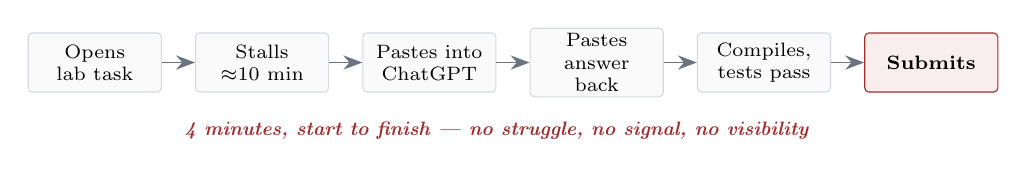
\begin{tikzpicture}[node distance=0.42cm]
    \node[wf] (s1) {Opens lab task};
    \node[wf, right=of s1] (s2) {Stalls\\ $\approx$10 min};
    \node[wf, right=of s2] (s3) {Pastes into\\ ChatGPT};
    \node[wf, right=of s3] (s4) {Pastes answer\\ back};
    \node[wf, right=of s4] (s5) {Compiles,\\ tests pass};
    \node[wf, right=of s5, draw=flag, fill=flag!8] (s6) {\textbf{Submits}};
    \foreach \a/\b in {s1/s2,s2/s3,s3/s4,s4/s5,s5/s6}{\draw[arr] (\a) -- (\b);}
    \node[lbl, below=0.30cm of s3.south east, text=flag]
      {\bfseries 4 minutes, start to finish --- no struggle, no signal, no visibility};
  \end{tikzpicture}
  \end{center}

  \vspace{0.9em}
  \begin{columns}[T]
    \begin{column}{0.31\textwidth}\stat{$+48\%$}{practice score, unguarded AI}\end{column}
    \begin{column}{0.31\textwidth}
      \begin{beamercolorbox}[wd=\textwidth,sep=5pt,center,rounded=true]{flagbox}
        {\Large\bfseries\color{flag}$-17\%$}\\[0.15em]{\scriptsize\color{muted}unaided exam score}
      \end{beamercolorbox}
    \end{column}
    \begin{column}{0.31\textwidth}\stat{$50\%$}{used the bypass button}\end{column}
  \end{columns}
  \vspace{0.35em}
  {\centering\scriptsize\color{muted}PNAS 2025, RCT, $n\approx$1{,}000\quad$\vert$\quad optional-guardrail study, $n{=}885$\par}

  \punchflag{The weakest students delegate most. \textbf{The harm is not uniform} --- and uniform assistance widens the gap it is meant to close.}
\end{frame}

%=======================================================================
% SLIDE 3 -- EXISTING SOLUTIONS
%=======================================================================
% SPEAKER SCRIPT (75 s) -- RAUF
% "We compared the closest published systems and the closest prior FYP here.
%  CodeHelp and CodeAid are guardrailed tutors at real scale -- CodeAid across
%  seven hundred students. Both give the same hint to every student, and neither
%  measured learning; CodeAid reports usage and perceptions only.
%  ClassAid, at CHI this year, is closest to us -- and still has no per-student
%  model. An instructor watches a dashboard and switches one of four modes for the
%  whole class.
%  Codio was approved here last year and I want to be precise, because it is well
%  built. Import a YouTube playlist; pause the video, Gemini extracts the code from
%  the frame, Judge0 runs it in a sandbox. But every AI feature it has hands the
%  learner code -- extraction, auto-completion, fix suggestions. Its adaptivity is
%  quiz difficulty from transcripts. Codio removes friction. We calibrate it.
%  Opposite objectives.
%  So the gap is precise. Everyone here has assistance. Nobody has a per-student
%  knowledge state to calibrate it against -- and nobody keeps that state honest
%  when the student delegates.  Zuhair."
% [STAGE] Deliver the Codio lines GENEROUSLY. Then three flat beats:
%         removes / calibrate / opposite. Then stop.
\begin{frame}{Where every existing system stops}
  \vspace{0.2em}
  \resizebox{\textwidth}{!}{%
  \begin{tabular}{@{}llllll@{}}
    \toprule
    \textbf{System} & \textbf{Per-student} & \textbf{Hint} & \textbf{Leakage} &
    \textbf{Compute /} & \textbf{Learning} \\
     & \textbf{knowledge model} & \textbf{calibration} & \textbf{control} &
    \textbf{residency} & \textbf{outcome measured} \\
    \midrule
    CodeHelp \textcolor{muted}{Koli '23}      & No & One-size-fits-all & Prompt guardrail & Cloud, off-prem & No \\
    CodeAid \textcolor{muted}{CHI '24, n=700} & No & One-size-fits-all & Pseudocode-only  & Cloud, off-prem & No --- usage only \\
    ClassAid \textcolor{muted}{CHI '26, n=54} & \alert{No} & Instructor picks 1 of 4 modes & Mode-based & Cloud, off-prem & No \\
    Codio \textcolor{muted}{FAST FYP '25}     & No --- quiz difficulty & \alert{None --- hands over code} & None & Cloud, off-prem & No \\
    \midrule
    \rowcolor{accent!14}
    \textbf{Scaffold} & \textbf{Yes --- BKT / DKT} & \textbf{Automatic, per student} &
    \textbf{Graduated + AST} & \textbf{Local 7B, on-prem} & \textbf{Yes --- transfer task} \\
    \bottomrule
  \end{tabular}}

  \vspace{0.8em}
  {\small\lead{The gap.} Everyone here has assistance. \textbf{Nobody has a per-student
  knowledge state to calibrate it against} --- and nobody keeps that state honest when
  the student delegates.\par}

  \punch{Codio is well built --- Gemini pause-to-code, Judge0 sandbox. But every AI feature \textbf{hands the learner code}.\\[0.15em]\textbf{Codio removes friction. We calibrate it. Opposite objectives.}}
\end{frame}

%=======================================================================
% SLIDE 4 -- R&D BASIS
%=======================================================================
% SPEAKER SCRIPT (65 s) -- ZUHAIR
% "Three sources drive our design decisions. The engineering takeaway from each,
%  not the summary.
%  Bastani, in PNAS. The finding is not that AI is harmful -- it is that the
%  guardrail is the load-bearing part. Same model, same students: unguarded, minus
%  seventeen percent on the unaided exam; guardrailed, minus point four, not
%  significant. So our guardrail inspects generated text on the output side, not a
%  line in a system prompt -- prompt-only guardrails collapse under sustained
%  adversarial pressure.
%  Deep Knowledge Tracing and its code-aware descendants. LSTMs over
%  skill-and-correctness tuples. Everything they observe is correctness. That input
%  vector is exactly where we intervene.
%  Third, and this shaped the project. A 2025 study poisoned BKT, AFM and DKT with
%  simulated gaming and measured up to a fifteen-point AUC collapse -- parametric
%  models worst hit. BKT is parametric. So BKT is our baseline to beat, not our
%  deployment model."
% [STAGE] Credibility slide. Do not hurry. Say "minus point four, NOT SIGNIFICANT"
%         -- correct statistical language, unprompted, is worth an extra slide.
\begin{frame}{Three findings, three design decisions}
  \vspace{0.5em}
  \renewcommand{\arraystretch}{1.55}
  \begin{tabular}{@{}p{0.30\textwidth}@{\hspace{0.4em}}c@{\hspace{0.4em}}p{0.55\textwidth}@{}}
    \lead{Bastani, PNAS 2025}\newline
    {\footnotesize\color{muted}$-17\%$ unaided exam unguarded;\newline $-0.4\%$ guardrailed (n.s.)}
    & {\color{accent}\Large$\Rightarrow$} &
    The guardrail is \textbf{load-bearing}. Ours inspects generated text
    \textbf{output-side}, not a line in a prompt. \\
    \lead{DKT / Code-DKT}\newline
    {\footnotesize\color{muted}LSTMs over (skill, correct)}
    & {\color{accent}\Large$\Rightarrow$} &
    Everything they observe is \textbf{correctness}. That input vector is where
    we intervene. \\
    \lead{Gaming \& learner modeling, 2025}\newline
    {\footnotesize\color{muted}up to \textbf{$-15.2\%$ AUC}, parametric worst}
    & {\color{accent}\Large$\Rightarrow$} &
    BKT is our \textbf{baseline to beat}, not our deployment model. Label
    corruption becomes an \textbf{evaluated condition}. \\
  \end{tabular}
  \punch{Every student model in this field observes only \textbf{whether the answer was right}.}
\end{frame}

%=======================================================================
% SLIDE 5 -- COMPLEX COMPUTING CHALLENGE
%=======================================================================
% SPEAKER SCRIPT (70 s) -- ZUHAIR
% "Why this is not a CRUD application or an API wrapper. Four constraints.
%  The first is the interesting one. Our estimator is adversarially corrupted by
%  design. A delegating student submits correct code, so a naive model raises their
%  mastery and gives them LESS help. And it compounds -- our own intervention
%  changes the student's behaviour, which changes the data the model learns from.
%  No stationarity, therefore no convergence guarantee. The loop feeds itself.
%  Second, real time. Sixty concurrent streams, p95 capture under two hundred
%  milliseconds, zero event loss. Events arrive out of order from async producers
%  and must be reconciled per student before scoring -- a race on the mastery update.
%  Third, static analysis of C++ that does not compile. Twenty-five percent of
%  incorrect submissions in the reference dataset. Precisely the struggling students.
%  Fourth, a hard bound: twenty-four gigabytes of VRAM, p95 under eight seconds at
%  ten concurrent, on-premises."
% [STAGE] Read only the four headers off the slide. Say the rest looking at the
%         PANEL. The final punch line is your Core-Replacement answer -- deliver it
%         slowly, then STOP and let it sit.
\begin{frame}{Four hard constraints}
  \vspace{0.6em}
  \begin{columns}[T]
    \begin{column}{0.48\textwidth}
      {\small\lead{C1 \ Adversarially corrupted estimation}\par\vspace{0.1em}
      Correct code is no longer evidence, and our own intervention changes the
      generating distribution.\par\vspace{0.15em}
      {\color{flag}\textbf{No stationarity $\Rightarrow$ no convergence guarantee.}}\par}
      \vspace{1.0em}
      {\small\lead{C3 \ Analysis of \emph{non-compiling} C++}\par\vspace{0.1em}
      \textbf{$\approx$25\%} of incorrect submissions never compile --- precisely the
      struggling students.\par}
    \end{column}
    \begin{column}{0.48\textwidth}
      {\small\lead{C2 \ Real-time ordered ingestion}\par\vspace{0.1em}
      60 concurrent streams, \textbf{$p_{95}<200$\,ms}, zero loss. Out-of-order events
      reconciled per student --- \textbf{a race on the mastery update}.\par}
      \vspace{1.0em}
      {\small\lead{C4 \ Bounded inference budget}\par\vspace{0.1em}
      $\le$24\,GB VRAM, INT4, \textbf{$p_{95}<8$\,s} at 10 concurrent,
      \textbf{on-premises}.\par}
    \end{column}
  \end{columns}
  \vspace{0.5em}
  {\centering\scriptsize\color{muted}Seoul Accord CCP characteristics 1--9\par}
  \punch{\textbf{Delete the language model entirely and all four problems are still there.}}
\end{frame}

%=======================================================================
% SLIDE 6 -- SOLUTION AND CONTRIBUTION
%=======================================================================
% SPEAKER SCRIPT (85 s) -- ZUHAIR
% "Here is the system. Telemetry streams from a Monaco editor over WebSocket --
%  Jawad built that layer.
%  Two consumers read the stream: a struggle detector, and a behaviour classifier
%  separating productive struggle from stuck from delegated. Both feed the
%  knowledge tracing engine, which maintains a per-concept mastery vector WITH
%  UNCERTAINTY ATTACHED. That vector plus the struggle signal selects a disclosure
%  level. Only then does the model render that level into English, and the guardrail
%  inspects the output before the student sees it.
%  Note the amber path. When the estimate is uncertain, we disclose LESS, not more.
%  Under-helping is recoverable. Over-helping destroys the thing we are protecting.
%  Three contributions. First, the closed loop -- telemetry, to knowledge state, to
%  calibrated disclosure, with no human in the real-time path. ClassAid needs an
%  instructor to switch modes; we compute the level.
%  Second, our primary research claim: telemetry-enriched DKT evaluated for mastery
%  VALIDITY under AI-mediated submissions, not just for AUC.
%  Third, a graduated AST-similarity leakage measure -- signature, naming,
%  pseudocode, partial, full -- generalising the binary leakage reward used in all
%  prior pedagogical-alignment work, which is entirely mathematics."
% [STAGE] Trace the diagram left to right with your hand. STOP your hand on the
%         amber box for the uncertainty line. This is the slide they remember --
%         if behind the clock, take the time from Slide 4, never from here.
\begin{frame}{The closed loop}
  \begin{center}
  \resizebox{0.84\textwidth}{!}{%
  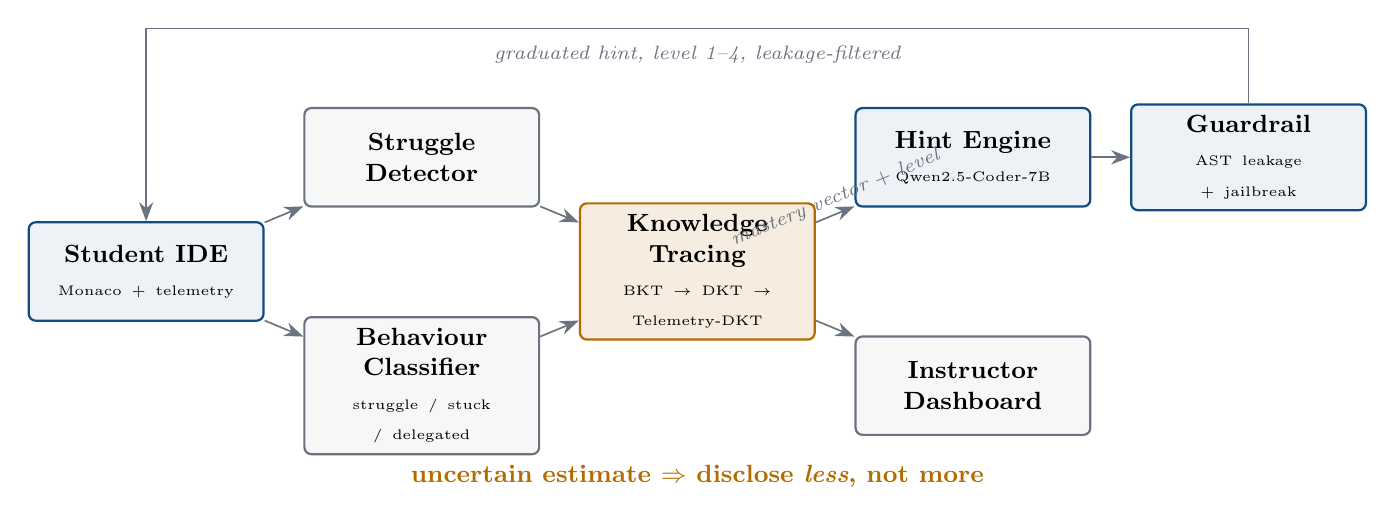
\begin{tikzpicture}
    \node[mod]    (ide)   at (0,0)      {Student IDE\\[1pt]{\tiny\mdseries Monaco + telemetry}};
    \node[modalt] (det)   at (3.5,1.45) {Struggle\\ Detector};
    \node[modalt] (cls)   at (3.5,-1.45){Behaviour Classifier\\[1pt]{\tiny\mdseries struggle / stuck / delegated}};
    \node[modnew] (kt)    at (7.0,0)    {Knowledge Tracing\\[1pt]{\tiny\mdseries BKT $\to$ DKT $\to$ Telemetry-DKT}};
    \node[mod]    (hint)  at (10.5,1.45){Hint Engine\\[1pt]{\tiny\mdseries Qwen2.5-Coder-7B}};
    \node[modalt] (dash)  at (10.5,-1.45){Instructor Dashboard};
    \node[mod]    (guard) at (14.0,1.45){Guardrail\\[1pt]{\tiny\mdseries AST leakage + jailbreak}};

    \draw[arr] (ide) -- (det);   \draw[arr] (ide) -- (cls);
    \draw[arr] (det) -- (kt);    \draw[arr] (cls) -- (kt);
    \draw[arr] (kt)  -- node[lbl,above,sloped,pos=0.66]{mastery vector $+$ level} (hint);
    \draw[arr] (kt)  -- (dash);
    \draw[arr] (hint) -- (guard);
    \draw[arr] (guard.north) -- ++(0,0.95) -| (ide.north);
    \node[lbl] at (7.0,2.75) {graduated hint, level 1--4, leakage-filtered};
    \node[lbl, text=amber, font=\small\bfseries] at (7.0,-2.6)
      {uncertain estimate $\Rightarrow$ disclose \emph{less}, not more};
  \end{tikzpicture}}
  \end{center}

  \vspace{0.25em}
  {\scriptsize
  \lead{1 \ Closed loop} --- \textcolor{muted}{no human in the real-time path. ClassAid needs an instructor to switch modes; we compute the level.}\par\vspace{0.1em}
  \co{2 \ Telemetry-DKT validated for \emph{mastery validity}, not AUC} --- \textcolor{muted}{\textbf{primary claim}: does behavioural signal keep the estimate honest when the code is not the student's?}\par\vspace{0.1em}
  \lead{3 \ Graduated AST leakage measure} --- \textcolor{muted}{prior work treats leakage as binary, and all of it is mathematics.}}
\end{frame}

%=======================================================================
% SLIDE 7 -- POC / FEASIBILITY
%=======================================================================
% SPEAKER SCRIPT (65 s) -- JAWAD, with handback to ZUHAIR
% JAWAD: "What runs today. Telemetry capture is live -- Monaco to WebSocket to
%  FastAPI, logging keystroke, paste and compile events while you type. The vLLM
%  serving check is reproduced inside the twenty-four gigabyte budget. And the
%  knowledge tracing pipeline executes: pyBKT fitted on CSEDM CodeWorkout, four
%  hundred and ten students in ProgSnap2 format, producing per-student mastery with
%  a reported AUC.  The risk experiment is Zuhair's."
% ZUHAIR: "We injected synthetic AI-mediated submissions into held-out trajectories
%  at twenty-five and fifty percent, and measured how far each model's mastery
%  estimate inflates. That is this chart. It tests the one assumption the whole
%  project rests on -- and if it had come out flat, we would be standing here
%  telling you our premise is wrong."
% JAWAD: "Not built: the disclosure policy, the guardrail, the dashboard, the C++
%  knowledge-component taxonomy, and the study."
% [STAGE] The handback is deliberate -- ownership without a slide change.
%         Jawad: say the NOT BUILT list fast and without apology.
\begin{frame}{What already runs}
  \vspace{0.4em}
  \begin{columns}[T]
    \begin{column}{0.53\textwidth}
      {\color{accent}\textbf{PROVEN TODAY}}\par\vspace{0.3em}
      {\small\begin{itemize}\setlength{\itemsep}{0.35em}
        \item \textbf{KT pipeline runs} --- pyBKT on CSEDM / CodeWorkout, 410 students.
        \item \co{Risk experiment} --- injection at 25\,\% / 50\,\%, inflation measured
              across all three models.
        \item \textbf{Telemetry live} --- Monaco $\to$ WebSocket $\to$ FastAPI;
              vLLM + INT4 verified inside 24\,GB.
      \end{itemize}}
      \vspace{0.5em}
      {\color{flag}\footnotesize\textbf{NOT BUILT YET}}
      {\footnotesize\color{muted}--- disclosure policy $\cdot$ guardrail $\cdot$ dashboard
      $\cdot$ C++ KC taxonomy $\cdot$ study}
    \end{column}
    \begin{column}{0.45\textwidth}
      \centering
      % ---- swap for the real chart before the defense: ----
      % \includegraphics[width=\linewidth]{poc_screenshot.png}
      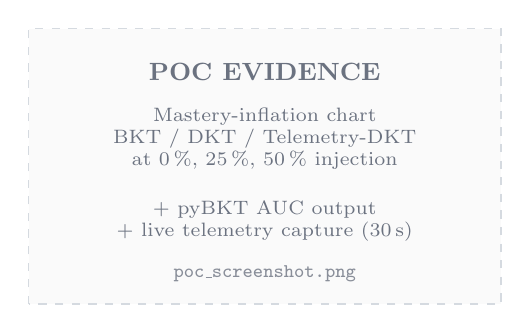
\begin{tikzpicture}
        \draw[dashed, semithick, rule, fill=black!2] (0,0) rectangle (6.0,3.5);
        \node[align=center, text=muted, font=\small\bfseries] at (3.0,2.95) {POC EVIDENCE};
        \node[align=center, text=muted, font=\scriptsize] at (3.0,2.10)
             {Mastery-inflation chart\\ BKT / DKT / Telemetry-DKT\\ at 0\,\%, 25\,\%, 50\,\% injection};
        \node[align=center, text=muted, font=\scriptsize] at (3.0,1.05)
             {+ pyBKT AUC output\\ + live telemetry capture (30\,s)};
        \node[align=center, text=muted!80, font=\scriptsize\ttfamily] at (3.0,0.38) {poc\_screenshot.png};
      \end{tikzpicture}
    \end{column}
  \end{columns}
  \punch{If the inflation had come out flat, \textbf{we would be telling you our premise is wrong}.}
\end{frame}

%=======================================================================
% SLIDE 8 -- EVALUATION AND RISKS
%=======================================================================
% SPEAKER SCRIPT (55 s) -- JAWAD
% "Evaluation. Deliberately NOT time-to-solution -- that is maximised by a system
%  that just gives the answer. Our pre-registered primary outcome is transfer-task
%  performance on an unaided task, with hint dependency across successive labs.
%  System targets: p95 capture under two hundred milliseconds at sixty users; hint
%  latency p95 under eight seconds at ten concurrent; DKT AUC at least point seven
%  under leave-students-out cross-validation; leakage below five percent at a sixty
%  percent AST-similarity threshold.
%  Two fallbacks matter. If the injection experiment shows no difference, our
%  premise is disproved -- we report that, and the closed-loop contribution still
%  stands. If Qwen's hint quality fails acceptance, we use a commercial API for the
%  study only and document the trade-off rather than hide it."
% [STAGE] Say "leave-students-out cross-validation" IN FULL. Anyone can say AUC;
%         the split is what proves you understand the evaluation.
\begin{frame}{How we will know}
  \vspace{0.4em}
  \begin{columns}[T]
    \begin{column}{0.50\textwidth}
      {\color{accent}\textbf{TARGETS}}\par\vspace{0.2em}
      {\scriptsize
      \begin{tabular}{@{}p{0.46\textwidth}@{}p{0.52\textwidth}@{}}
        \textbf{Primary outcome} & Transfer task, \emph{unaided} \\[0.28em]
        \co{Mastery inflation} & \co{Telemetry-DKT $<$ DKT $<$ BKT} \\[0.28em]
        DKT accuracy & AUC $\ge0.70$, \emph{leave-students-out} \\[0.28em]
        Capture / hint latency & $p_{95}<200$\,ms \ $\vert$ \ $p_{95}<8$\,s \\[0.28em]
        Leakage & $<5\%$ at AST sim.\ $\ge60\%$ \\[0.28em]
        Study & $n\ge30$, $\alpha{=}0.05$, $\beta{=}0.80$ \\
      \end{tabular}}
    \end{column}
    \begin{column}{0.47\textwidth}
      {\color{flag}\textbf{IF IT FAILS}}\par\vspace{0.2em}
      {\scriptsize
      \begin{itemize}\setlength{\itemsep}{0.45em}
        \item \textbf{Injection experiment flat} $\to$ premise disproved. We report
              it; the closed-loop contribution stands.
        \item \textbf{Qwen quality too low} $\to$ commercial API for the study only,
              trade-off documented, not hidden.
        \item \textbf{KC taxonomy slips} $\to$ transfer learning from correctness labels.
        \item \textbf{DPO fails} $\to$ secondary track; a reportable negative result.
      \end{itemize}}
    \end{column}
  \end{columns}
  \punch{Deliberately \textbf{not} time-to-solution --- that metric is maximised by a system that just gives the answer.}
\end{frame}

%=======================================================================
% SLIDE 9 -- WORK DIVISION
%=======================================================================
% SPEAKER SCRIPT (40 s) -- JAWAD
% "Each of us owns a subsystem that disappears if we are removed -- and defends it
%  here today. Zuhair owns knowledge tracing and mastery validity. I own real-time
%  capture: telemetry pipeline, struggle detector, latency and concurrency, and the
%  instructor dashboard. Rauf owns disclosure and evaluation -- the hint generation
%  path, the C++ knowledge-component taxonomy, the ethics application, and the
%  classroom study.
%  Semester one closes at roughly forty-five percent implemented. The two items most
%  likely to slip -- ethics approval and the taxonomy -- are scheduled FIRST, in
%  month one."
\begin{frame}{Who owns what}
  \vspace{0.15em}
  \begin{columns}[T]
    \begin{column}{0.31\textwidth}
      \lead{Muhammad Zuhair}\par{\scriptsize\color{muted}23I-0001 \ $\vert$ \ ML}\par\vspace{0.4em}
      {\footnotesize Knowledge tracing \& \textbf{mastery validity}\par\vspace{0.3em}
      {\scriptsize\color{muted}BKT baseline $\cdot$ DKT comparison $\cdot$ injection experiment $\cdot$ Telemetry-DKT $\cdot$ DPO}}
    \end{column}
    \begin{column}{0.31\textwidth}
      \lead{Muhammad Jawad Ali}\par{\scriptsize\color{muted}23I-3024 \ $\vert$ \ Systems}\par\vspace{0.4em}
      {\footnotesize Real-time capture, \textbf{latency \& concurrency}\par\vspace{0.3em}
      {\scriptsize\color{muted}Telemetry pipeline $\cdot$ struggle detector $\cdot$ integration $\cdot$ instructor dashboard}}
    \end{column}
    \begin{column}{0.31\textwidth}
      \lead{Abdul Rauf}\par{\scriptsize\color{muted}23I-0591 \ $\vert$ \ Full-stack \& Research}\par\vspace{0.4em}
      {\footnotesize Disclosure policy, \textbf{leakage \& evaluation}\par\vspace{0.3em}
      {\scriptsize\color{muted}Hint generation $\cdot$ C++ KC taxonomy $\cdot$ ethics $\cdot$ guardrail $\cdot$ classroom study}}
    \end{column}
  \end{columns}

  \vspace{0.45em}
  \begin{center}
  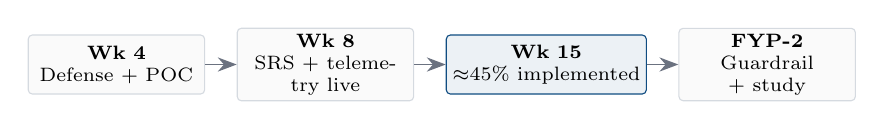
\begin{tikzpicture}[node distance=0.4cm]
    \node[wf, text width=2.1cm] (w4) {\textbf{Wk 4}\\ Defense + POC};
    \node[wf, text width=2.1cm, right=of w4] (w8) {\textbf{Wk 8}\\ SRS + telemetry live};
    \node[wf, text width=2.4cm, right=of w8, draw=accent, fill=accent!8] (w15) {\textbf{Wk 15}\\ $\approx$45\% implemented};
    \node[wf, text width=2.1cm, right=of w15] (s2) {\textbf{FYP-2}\\ Guardrail + study};
    \foreach \a/\b in {w4/w8,w8/w15,w15/s2}{\draw[arr] (\a) -- (\b);}
  \end{tikzpicture}
  \end{center}

  \punch{The two items most likely to slip --- \textbf{ethics approval and the KC taxonomy} --- are scheduled \textbf{first}, in month one.}
\end{frame}

%=======================================================================
% SLIDE 10 -- DEI, ETHICS, LEGAL
%=======================================================================
% SPEAKER SCRIPT (45 s) -- RAUF
% "Finally -- and for this project these are not boilerplate.
%  On equity: the bypass study showed the weakest students delegate most. A mastery
%  model accurate only for strong students would widen exactly the gap we exist to
%  close. So we report knowledge-tracing performance disaggregated by prior
%  programming exposure, and publish any disparity rather than omit it.
%  On ethics: consent before any collection, ethics application in month one,
%  university-controlled storage, grade independence in writing. The model runs
%  on-premises -- student code never leaves campus.
%  And Scaffold never accuses anyone. It surfaces signals to a human. A false
%  suspicion is real harm to a student, so we treat it as a design constraint, not
%  an edge case."
% [STAGE] Slow down here. This is the last thing they hear before questions.
\begin{frame}{DEI, ethics, legal}
  \vspace{0.6em}
  \begin{columns}[T]
    \begin{column}{0.33\textwidth}
      \lead{Equity}\par\vspace{0.3em}
      {\footnotesize The weakest students delegate most. A model accurate only for strong
      students \textbf{widens the gap it exists to close}.\par\vspace{0.4em}
      {\footnotesize\color{muted}KT performance reported disaggregated by prior programming
      exposure --- \textbf{disparity published, not omitted}.}}
    \end{column}
    \begin{column}{0.33\textwidth}
      \lead{Ethics}\par\vspace{0.3em}
      {\footnotesize Consent before any collection. Ethics application \textbf{Month 1}.
      University-controlled storage. Grade independence in writing.\par\vspace{0.4em}
      {\footnotesize\color{muted}Local 7B model --- \textbf{student code never leaves campus}.}}
    \end{column}
    \begin{column}{0.33\textwidth}
      \lead{Legal / IP}\par\vspace{0.3em}
      {\footnotesize Qwen2.5-Coder-7B, vLLM \textbf{Apache 2.0}. pyBKT, PyTorch-DKT, Monaco
      \textbf{MIT}.\par\vspace{0.4em}
      {\footnotesize\color{muted}CSEDM under its research data-use agreement. Commercial
      APIs: development only, never deployed.}}
    \end{column}
  \end{columns}
  \punchflag{\textbf{Scaffold never accuses anyone.} It surfaces signals to a human. A false suspicion is real harm to a student --- a design constraint, not an edge case.}
\end{frame}

%=======================================================================
% CLOSING
%=======================================================================
% SPEAKER SCRIPT (10 s) -- RAUF
% "Adaptive help needs a student model. Every student model is computed from
%  submission correctness. Delegation breaks that measurement -- and repairing it is
%  our contribution.  Thank you. We'll take questions."
% [STAGE] Land it, say thank you, STOP TALKING, stand still. No "that's it".
\begin{frame}[plain]
  \vspace{1.6cm}
  \begin{center}
    {\color{accent}\rule{2.6cm}{2.2pt}}\par\vspace{0.6em}
    {\fontsize{26}{30}\selectfont\bfseries\color{ink}Thank you}\par\vspace{0.3em}
    {\large\color{muted}Questions}\par\vspace{1.1em}
    \begin{minipage}{0.80\textwidth}
      \begin{beamercolorbox}[wd=\textwidth,sep=9pt,rounded=true]{punchbox}
        \centering Adaptive help needs a student model. Every student model is computed
        from \textbf{submission correctness}. \textbf{Delegation breaks that
        measurement} --- and repairing it is our contribution.
      \end{beamercolorbox}
    \end{minipage}\par\vspace{1.0em}
    {\scriptsize\color{muted}Muhammad Zuhair \ $\vert$ \ Muhammad Jawad Ali \ $\vert$ \ Abdul Rauf\\
     Supervisor: Ma'am Rabail Zahid \ $\vert$ \ FAST NUCES Islamabad}
  \end{center}
\end{frame}

\end{document}
